\documentclass{article}
\usepackage[utf8]{inputenc}
\usepackage[margin=1.0in]{geometry}
\usepackage[bottom]{footmisc}
\usepackage{graphicx}
\usepackage{hyperref}
\usepackage{mathtools}
\usepackage{amsmath}
\usepackage{tcolorbox}
\usepackage{subcaption}
\usepackage{float}
\usepackage{multirow}
\usepackage{titlesec}
\setcounter{secnumdepth}{4}
\usepackage[toc,page]{appendix}

\title{Discussion Section}
\date{June 2020}

\begin{document}

\maketitle

\section{General Technique Discussion}

\subsection{MCMC}
While there are many implementations of MCMC algorithms, parameterizing with Metropolis and DRAM MCMC methods has helped us understand the power and performance of a small subset of these algorithms. Our findings tell us that the Metropolis algorithm is suitable for simple systems with relatively small numbers of parameters and that DRAM will perform comparably or better on such systems. However, when system complexity and parameter space increases, we find that the DRAM algorithm outperforms the simple Metropolis method. 
\par We have also discovered that there is no universal rule in determining the validity of results. Through our implementation process we have determined 3 main techniques to confirm valid and accurate results
\begin{enumerate}
    \item Chain mixing and convergence
    \item Visual validation
    \item Statistical validation
\end{enumerate}
\subsubsection{Metropolis vs. DRAM}
While we cannot make any formal, general claims about the difference in performance of both algorithms, we have found that of the two methods - Metropolis and DRAM MCMC, the Metropolis method tends to perform well on simpler systems with a small number of parameters while the DRAM MCMC method can be used on more complex systems with a larger number of parameters. We hypothesize that this difference is due to the way in which each algorithm deals with a rejected candidate set. Recall in the simple Metropolis method that we sample a  candidate under specific conditions and if that candidate is rejected, we update the sampling conditions and move on to the next candidate. In the DRAM method however, if we reject a candidate, before updating any sampling conditions, we sample alternative candidates using the same conditions. This pause in updating allows the algorithm to search more extensively in spaces of lower probability and helps prevent the algorithm from getting stuck in local maxima as the Metropolis is known to do. \par Now let's think about what this means in the context of simple and complex models. In the case of the Lotka-Volterra model, the parameter space is relatively small and using the Metropolis method we are likely to be able to search the whole parameter space without getting stuck in local maxima. However, in the Type 1 Diabetes model, our parameter space increases exponentially. Now there is a higher probability of correlation between parameters (recall parameter identifiability in Section XXX) and a higher chance that the Metropolis method will get stuck in local maxima.
\subsubsection{Validation Techniques}
Current literature points to several evaluation techniques including chain convergence diagnostics such as Geweke's diagnostic and chain acceptance rate, both of which we have discussed in terms of our results. However, we are cautious to use any single technique alone to determine the validity of our results. We have found that using several techniques in tandem has helped us get a better understanding of the performance of our algorithm and to make a decision as to the accuracy of its results. \vspace{4 mm}

\underline{Chain mixing and convergence:} Both the Metropolis and DRAM MCMC methods rely on sampling with which we hope to choose the best sets of parameters for our model. Because of the importance of sampling, we want to determine that our chain is actually sampling is well-mixed so that we eventually reach the best range of values for our parameters. To do this we have relied on a visual validation of chain convergence and mixing as well as the formal technique, Geweke's diagnostic, to determine convergence. Below we show examples of chain mixing\\
\begin{figure}[H]
\begin{subfigure}{.5\textwidth}
  \centering
  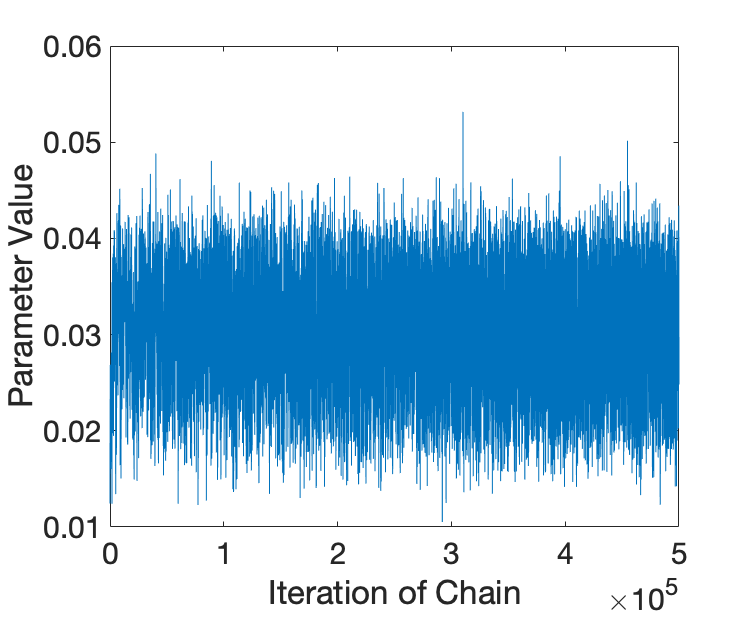
\includegraphics[width=.8\linewidth]{MCMC_figs/chain_mix_ex1.png}
  \caption{Example of a well-mixed chain.}
  \label{fig:sfig1}
\end{subfigure}%
\begin{subfigure}{.5\textwidth}
  \centering
  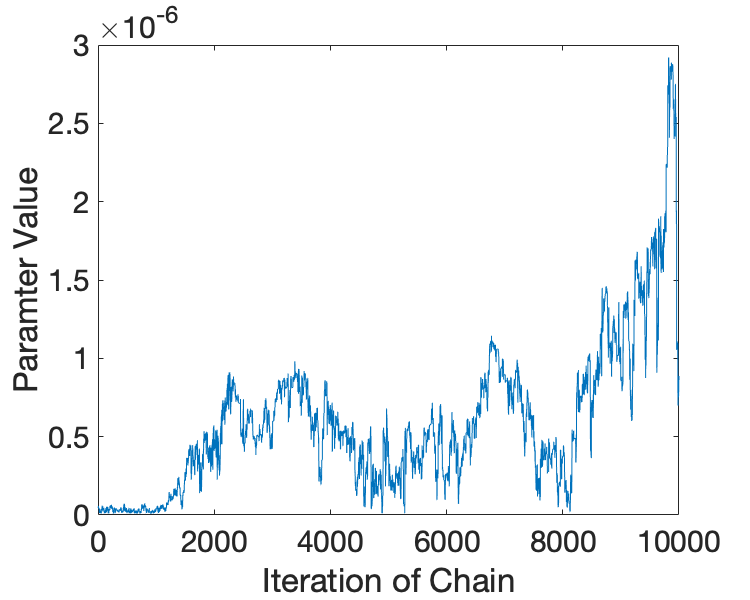
\includegraphics[width=.8\linewidth]{MCMC_figs/chain_mix_ex2.png}
  \caption{Example of a poorly-mixed chain.}
  \label{fig:sfig2}
\end{subfigure}
\centering
\begin{subfigure}{.5\textwidth}
  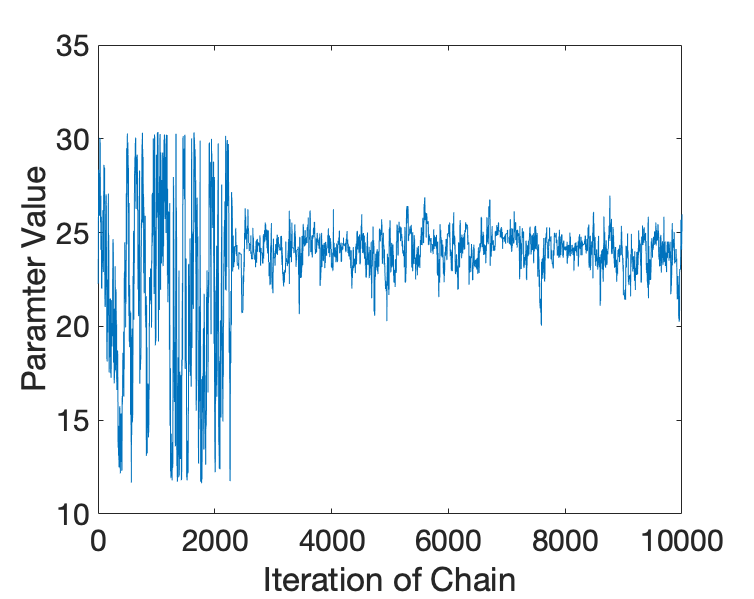
\includegraphics[width=.8\linewidth]{MCMC_figs/chain_mix_ex3.png}
  \caption{Example of a chain with a shift in mean.}
  \label{fig:sfig2}
\end{subfigure}
\caption{Comparing mixing of chains. Chain (a) was taken from the DRAM parameterization of the Lotka-Volterra model, parameter $\beta$. Chains (b) and (c) were taken from the Metropolis parameterization of the Type 1 Diabetes model, parameters e1 and $\beta_\eta$.}
\label{fig:fig}
\end{figure}
In 1(a), the chain is well-mixed, appears dense with evenly distanced samples, and even has a visually discernible constant mean. This indicates that our algorithm is properly sampling the parameter space. This visual analysis also tell us that it is highly likely that our chain has satisfactorily converged as the mean appears relatively constant throughout the sampling iterations. The chain in 1(b) does not appear well-mixed as its samples are not evenly distanced. We can even see that the mean is constantly changing which tells us that the chain has likely not converged for this parameter. Finally we can see an example of an abrupt change in mean (1(c)). We note that the chain starts out fairly well mixed, but around 4,000 samples, the mean shifts dramatically. The remaining samples are also fairly well-mixed, however the shift in means has impeded convergence and from the Geweke diagnostic, it is likely that this chain has not converged. However, this chain may be suggesting that the algorithm requires a longer burn-in period. For all our results, we confirmed the convergence of chains using both a visual and formal test.\vspace{4 mm}
\underline{Visual Validation:} Visual analysis of results is often considered an informal method of validation. However have found that a visual assessment of the results has allowed us to discard results that are not feasible for our model and focus on analyzing results that are. For, example when plotting glucose predictions in Section XXX, when we looked for a specific behavior in the prediction: a steady increase of glucose, an abrupt spike, and a levelling off. If we did not see this shape, we updated our algorithm. When comparing results from different runs, in the case that we cannot determine by eye which has produced the best results, we then turn to formal statistical validation techniques.\vspace{4 mm} \\
\underline{Formal Validation:} Common standards of formal validation include computations such as mean squared error (MSE) and standard estimate of error (SEE). Throughout the analyses of our results, we have chosen to use a root MSE score to compare and judge accuracy of results. This kind of score tell us how evaluations of our model using algorithm parameters differ from our raw data and provide us general insight into the goodness of fit of our parameterization. \vspace{3 mm} \\

We have found that using these 3 methods of validation together have helped us to determine whether or not our results are biologically feasible and to judge the overall performance of our algorithms. We caution that these techniques may not work for all biological models due to differences in parameter and model interactions, but we hope that it gives the reader a better foundation for determining their own methods. More generally, we recommend the use of multiple techniques as opposed to a single one, with the hopes that more information can be gathered as more techniques are used.
\subsubsection{Improvements Moving Forward}
We have been successful in creating a preliminary implementation of the DRAM MCMC algorithm for the Type 1 Diabetes model, however we acknowledge that there are some fixes that should be implemented in the future.
\begin{enumerate}
    \item Number of parameters
    \item User-specified functions
\end{enumerate}
\vspace{3 mm}
\underline{Number of parameters:} Although the findings from the UKF algorithms indicated that allowing all parameter values to vary at least slightly improves parameterization, we were unable to do this for the DRAM MCMC method. While running our DRAM MCMC algorithm on the Type 1 Diabetes model, we have used numerous different subsets of parameters. We have noticed that by increasing the number of parameters, our algorithm seems to reject more candidates. We hypothesize that as our parameter space becomes exponentially large, our current algorithm is unable to efficiently explore it. Therefore, we cannot yet run the algorithm on all 53 parameters as the chain acceptance rate essentially becomes 0\%. After experimenting with parameter subsets of different sizes, we hypothesize that our program could successfully paramterize around 10-20 parameters. However, the MCMC algorithms are meant to be able to parameterize complex systems with many parameters, so we hope that future work on our implementation will be able to incorporate a greater number of these parameters.\vspace{3 mm}\\

\underline{User-specified functions:} One of the reasons that MCMC is widely used is because of its ability to parameterize given no \textit{a priori} information. However, the \texttt{mcmcstat} library that both our implementations of the Metropolis and DRAM MCMC algorithms utilize allows users to specify their own functions, such as the prior function, depending on the \textit{a priori} information that they have available. We did an very basic implementation of a log-normal uniform prior (the process and results of which can be seen in Section 2 of this Discussion). This implementation of an informative prior was used primarily to test out the reaction of the MCMC parameterization with the incorporation a different prior. In the future a different implementation of this prior function should be considered and tested. 
\subsection{UKF}
\subsubsection{Findings}
Implementing both the Joint and Dual UKF algorithms on the Lotka-Volterra and T1D systems has given us a range of situations to consider in developing our general conclusions about these algorithms. We have made three main conclusions through our experiences:
\begin{enumerate}
    \item The importance of tuning algorithm parameters, including initial guesses.
    \item The Dual UKF is the superior approach.
    \item Underlying models determine the limits of the algorithm's success.
\end{enumerate}
Let us consider each of these points individually now.

\paragraph{Importance of Tuning}
No matter which algorithm or system we worked with, the largest portion of our effort was directed towards tuning the UKF's parameters, such as noise and state covariances and initial guesses. Thus, one should not expect to simply implement the algorithm and have quality results on the first attempt. As a result, understanding the inner-workings of the UKF's is essential. For example, understanding the connection between an increased state covariance and an increased Kalman Gain can be crucial if Kalman Gains are consistently too small while troubleshooting. As a result, one must spend adequate time with the theory before entering into the code. Additionally, much of previous literature has not emphasized enough the role of initializing the state estimate and covariance, namely $\hat{x}_0$ and $P_0$. However, our experiences have revealed that initialization of $\hat{x}_0$ and $P_0$ determine the \emph{region of parameter space} the algorithm searches. Thus, the initialization of the filter, particularly $P_0$, must be given the proper amount of attention.

\paragraph{Superiority of the Dual UKF}
Across both the Lotka-Volterra and T1D systems, the Dual UKF has been more successful when analyzed both visually and quantitatively. This is evidenced by Figures \ref{fig:LV_Dual_ODESims} and \ref{fig:LV_Joint_ODESims} for Lotka-Volterra, where we see the Dual's better performance when simulating the final ODEs, as well as in table \ref{table:LV_ODESims_RMSE}. Similarly, for T1D we look to Figures \ref{fig:T1D_Dual_AllAcute_Plots} and \ref{fig:T1D_Joint_AllAcute_Plots} for visualizations of the fits for the Dual and Joint respectively, as well as their corresponding Tables \ref{table:T1D_Dual_AllAcute_RMSE} and \ref{table:T1D_Joint_AllAcute_RMSE}. Thus, when approaching a new problem, we recommend beginning with the Dual UKF due to the superior results we witnessed from both a visual and quantitative standpoint. \\
\\
To understand why we see this discrepancy, consider the advantage the Dual provides us. The benefit of separating out noise and covariances between states and parameters appears to be more important than having covariance between states and parameters (as is the case in the Joint). Although previous experimentation has showed little difference in performance of the two approaches, we have seen Dual superiority on both systems \cite{GoveHollingerDual}.

\paragraph{Importance of the Underlying Model}
When working to parametrize a model to fit a particular dataset, the structure of the model you are working plays a large role in determining the limitations of the parametrization's success. By this, we mean that the relationships between states assumed in the ODEs, as well as the number and types of parameters (i.e. their biological significant), must be considered when assessing results. For example, the Lotka-Volterra model is a periodic model that assumes constant parameters through all the different cycles. Therefore, the model assumes that peaks and troughs for a particular population are consistent values and that spacing between peaks is constant. However, these assumptions do not always hold up with real data, since there are more parameters in play than the ones in the model. Thus, when presented with a dataset where peaks \emph{are not} consistently spaced, one should not expect to be able to fit this behavior with one constant set of parameters. On the other hand, the T1D model is a steady state system that is expected to follow a general path and eventually reach a steady state. The parameters of the system control the path the system takes, such as the set of parameters, $\alpha_\eta$, $\beta_\eta$, and $\eta$, that are designed to control the time and slope of disease onset. Thus, this behavior \emph{is} something one should expect to be able to fit to and should consider when looking at the parametrization's results. In general, model building and parametrization of said model should not be seen as independent tasks but are rather directly dependent on one another.

\subsubsection{Improvements Moving Forward} \label{section:UKF_FutureImprovements}
Although successful, the UKF methods we have implemented have room for improvement moving forward as they continue to be applied to the T1D model. There are three particular areas that we have identified:
\begin{enumerate}
    \item Understanding of Parameter Covariances as more iterations of the algorithm are run.
    \item Automation of noise calculations
    \item Improving biological accuracy of parameter estimates
\end{enumerate}
Let's begin with our first point.
\paragraph{Improvements to Parameter Covariances}
Referring back to figure \ref{fig:T1D_CodeFlow}, we see that the UKF algorithms are run 5 times on the T1D system and then the best run is chosen as the final representative. As we noted earlier, we choose the best of the 5 runs because the 5th is by no means guaranteed to perform best. This begs the obvious question: why does performing more iterations worsen the results? Our hypothesis is that it comes back to our decision of keeping initial parameter covariances constant across runs. This initial value, which is quite high, results in searching more of parameter space then we'd like after multiple iterations. Ideally, after one iteration is complete, we'd be more confident in the area of parameter space we are in, and thus would narrow our search space, and continue narrowing the search space until parameters converged. Visually, figure \ref{fig:Discussion_UKF_ChangingVariances} shows our current approach (top) versus our ideal one (bottom). In order to implement the approach, we need to determine a manner in which to decrease parameter covariances as more iterations occur. One possible solution is to simply multiply the starting variances by some constant value, for example 0.8, each time. This is likely to be a good starting point but we imagine this problem requires further analysis.

\begin{figure}[H]
    \centering
    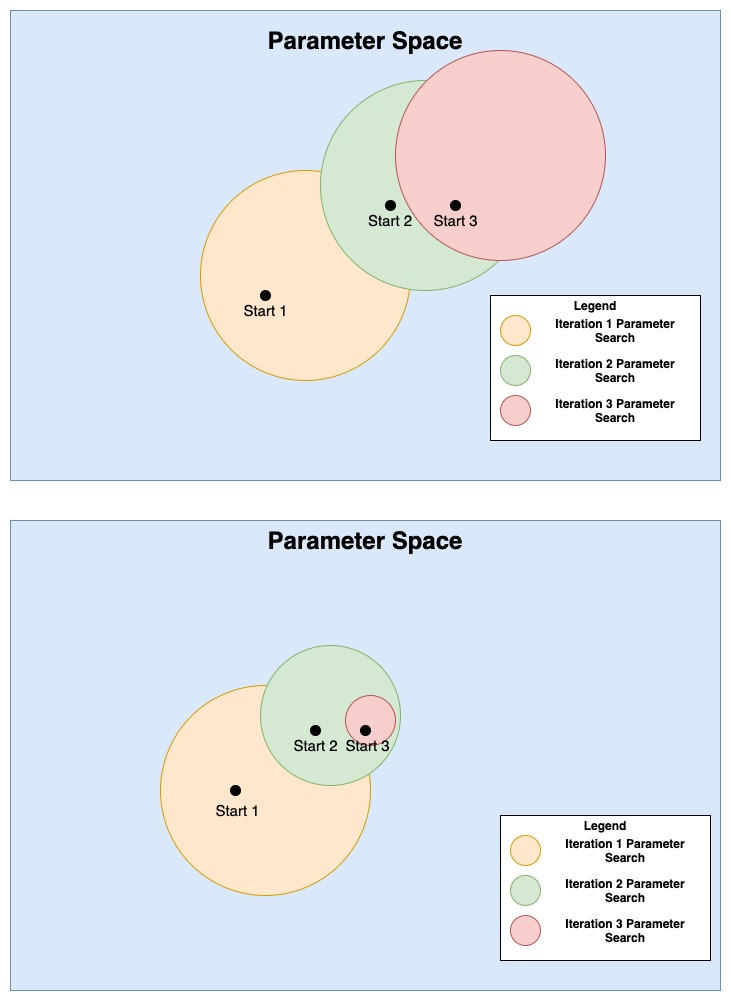
\includegraphics[width=15cm]{Kalman Filter Images/Decreasing_Param_Space .jpg}
    \caption{Visual depiction of proposed approach to decrease parmaeter search space as more iterations occur. On the top we continue to search a large area instead of narrowing our space in order to eventually reach convergence, as is done on the bottom. We hypothesize that this approach could improve future results.}
    \label{fig:Discussion_UKF_ChangingVariances}
\end{figure}

\paragraph{Automation of Noise Calculation}
An understanding of process and measurement noise has been essential to producing accurate fits to both the Lotka-Volterra and T1D datasets. Throughout \emph{Kalman Filter Implementation}, we have described methods found to work to calculate these noises, however they have only been successfully implemented in certain scenarios and sometimes only for the Dual or Joint. As a result, a large portion of time has been spent on manually tuning the amount of noise introduced in the algorithm in an ad hoc fashion. Although this will eventually produce satisfactory results, it is not ideal for two reasons. First, the time factor. The time spent on tuning parameters, although useful in gaining an intuitive understanding of the algorithms and improving performance, can be better spent working on other aspects of the UKF. Second, there is no guarantee that we have reached optimal noise values. Using ad hoc methods can lead to "good" fits, however whether there is a better one out there cannot be known unless algorithmic techniques are implemented to determine the amount of noise one should add to the system being simulated.

\paragraph{Improving biological accuracy of parameter estimates}
As discussed earlier, one of the most important things to consider when trying to paramaterize a biological system is whether the estimated parameters make biological sense. This means that the values of the parameters are within reasonable ranges and that when the system is run with these parameters, the results make biological sense as well. For the T1D system, as we discussed earlier, the parameters are supposed to live on the edge with two steady states, such that when the system is run with an apoptotic wave the mice become diabetic, but when there is no wave the mouse reaches a healthy steady state. Currently when our system is run, as shown in Figures \ref{fig:T1D_StatesNoWave} and \ref{fig:T1D_StatesWithWave} the mouse becomes diabetic in both scenarios. Further work would seek to explore why this is the case and tune the filter so that the resulting parameters do create the desired biological result. 

\subsection{PSO}


\section{Combining UKF and MCMC Methods} \label{section:Combining_UKF_MCMC}
Overall, we believe that we have had a satisfactory amount of success parameterizing the Type 1 Diabetes Model using the UKF, MCMC, and PSO methods individually. However, our teams note the potential of using the MCMC and UKF methods together with the hopes of creating an even more informed parameterization technique. We believe this can be achieved by providing the MCMC algorithms with an informative prior through use of the Dual UKF algorithm. Note that we utilize the Dual approach here due to it having more success on individual mice than its Joint counterpart. 


\subsection{Producing Prior Parameter Distributions}
An uninformative, log-uniform prior was used for all the results presented in the MCMC section (Section XXX). However the \texttt{mcmcstat} library allows the user to specify a unique prior function. When we have \textit{a priori} information about our system, we can incorporate this knowledge into the MCMC method using an informative prior. In order to provide the MCMC algorithm with an informative prior, we ran the Dual UKF on each of the 9 acute mice individually. Then, we fit normal distributions to these 9 data points for each parameter in the notable parameter subset as described in section \ref{section:Notable_parameter_subset}. The use of a \emph{normal distribution} is a large assumption, and one that is likely to be having a negative impact on our performance. For now, fitting normal distributions provides a simple solution that allows us to test the overall process of combining the UKF and MCMC techniques into a single method. Moving forward, more thought must be given to what distributions would fit the histograms below best. Additionally, it is important to consider that these distributions are relying on solely 9 datapoints. We consider this to be far too low of a sample size to produce trustworthy distributions. Thus, it will be important to develop methods to have access to more datasets moving forward. Figure \ref{fig:Discussion_UKFParamDistributions} displays histograms for each parameter in the notable parameter subset.

\begin{figure}[H]
    \centering
    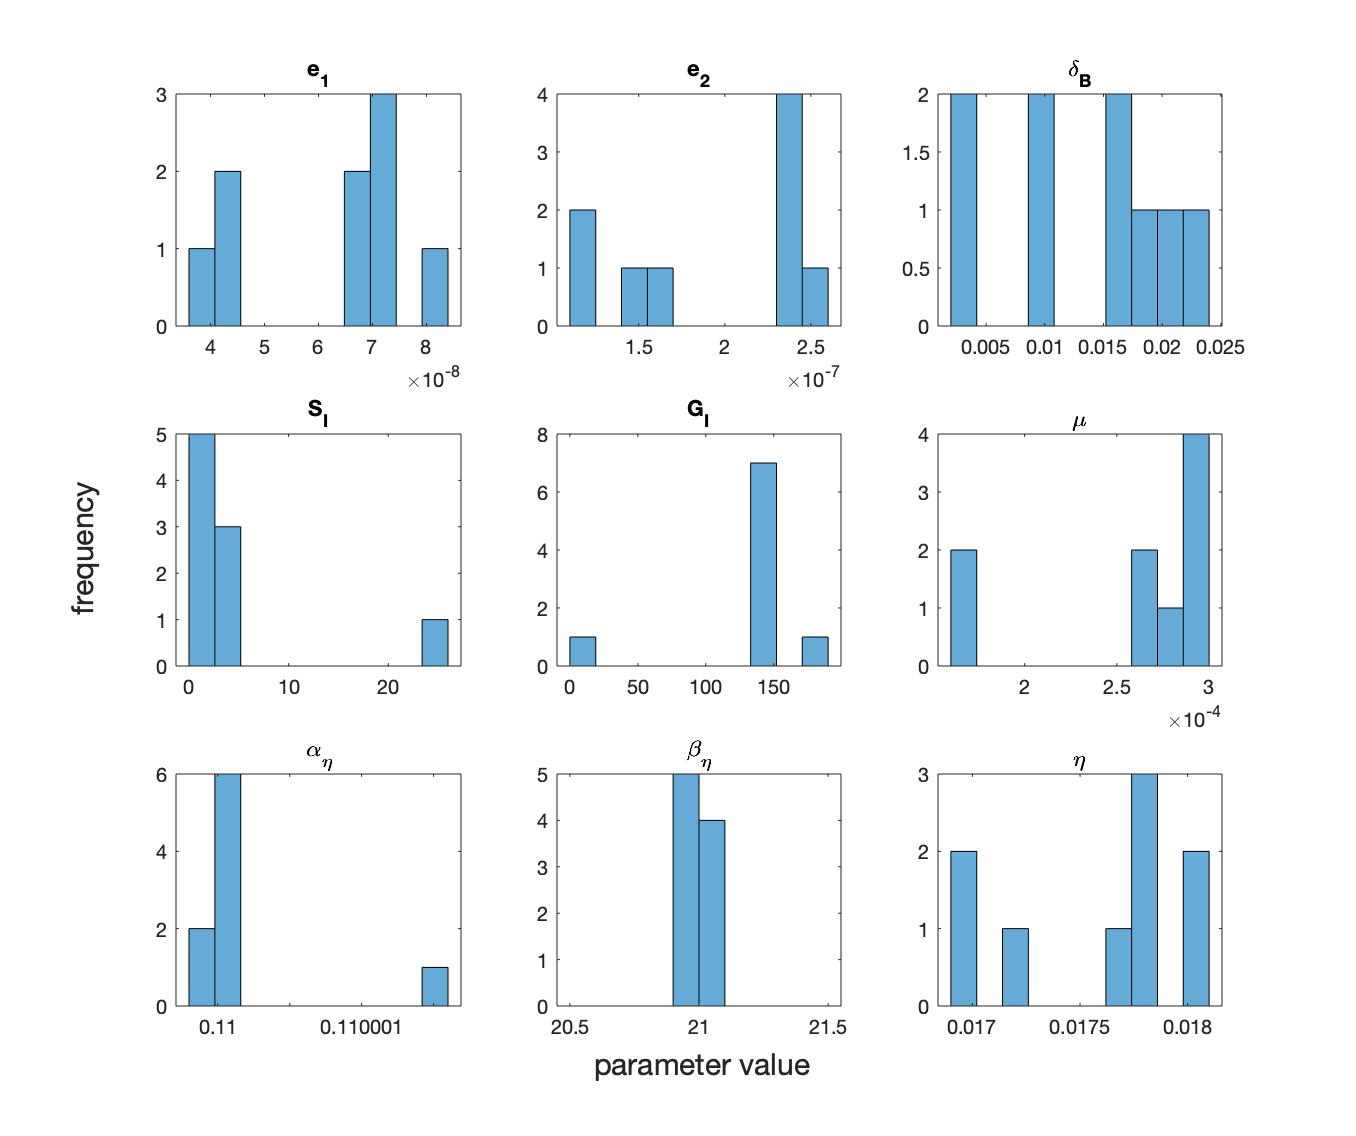
\includegraphics[width=15cm]{Comparison_Figures/Key_Parameter_Distributions.jpg}
    \caption{Histogram of distributions for key parameters created by running the Dual UKF on the 9 Li et al acute mice. There do not appear to be clear distributions that can be fit and, additionally, multiple parameters seem to show no clear mode in their histograms.}
    \label{fig:Discussion_UKFParamDistributions}
\end{figure}

Visually, it is clear that there is likely a range of distributions that would provide best fits for these parameters, something which would need to be done on a parameter-by-parameter basis. 

\subsection{Using an Informative Prior}
Using the normal distributions provided by the UKF algorithm required us to write our own prior function. Because of the conditions of the script that performs the DRAM sampling algorithm, we implemented a log-normal prior function (log form is specified by the \texttt{mcmcstat} library). We then parameterized the Type 1 Diabetes model using this informative prior on the averaged acute data. Below we compare the glucose predictions for a parameterization with and without an informative prior.
\begin{figure}[H]
    \centering
    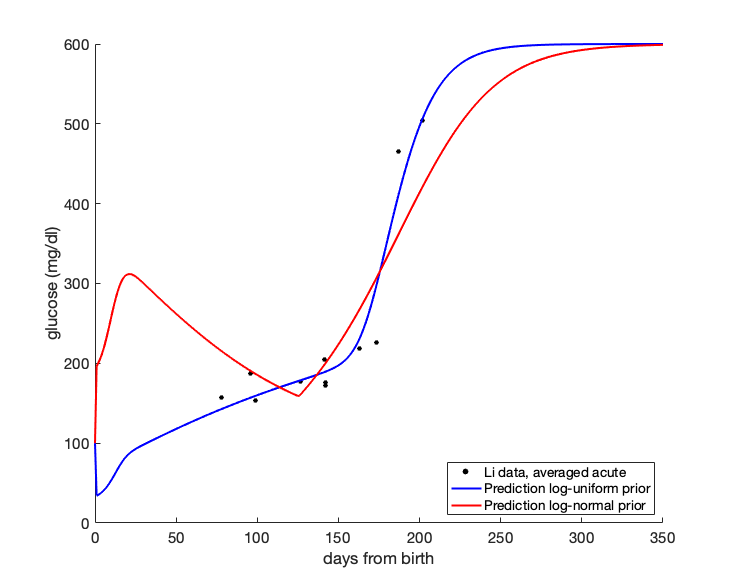
\includegraphics[width=15cm]{Comparison_Figures/dram_priorComp.png}
    \caption{Comparison of predictions when using log-normal and log-uniform prior functions. The averaged acute glucose data is plotted against the comparison. We can see that the use of an informative prior seems to have an impact on the beginning behavior of the prediction, however the end behaviors are more similar.}
\end{figure}
From this figure we can see that the informative log-normal prior does have an impact on the final parameter results. While the prediction with an log-uniform prior shows the steady increase and then sharp spike in glucose, in the prediction with the log-normal prior begins with a sharp spike before decreasing and spiking again. The most drastic differences we see between the two predictions are in the starting behaviors, onset times, and post-onset time slopes. It is unclear to us why the log-normal prior prediction produces an immediate increase and decrease in glucose instead of the expected steady increase to diabetes onset. It is clear that the uninformative, log-uniform prior produces better results. To formally compare the two results, we quantify the differences between glucose predictions using RMSE scores
\begin{table}[H]
  \begin{center}
    \label{tab:table1}
    \begin{tabular}{c|c} 
      \textbf{Prior Function} & \textbf{RMSE} \\
      \hline
      \textbf{Log-uniform} & 30.7\\
      \textbf{Log-normal} & 58.1\\
    \end{tabular}
    \caption{Root Mean Squared Error (MSE) of ODE simulations using a log-normal and log-uniform prior function. The root MSE scores confirm the our visual hypothesis that the log-uniform (uninformative) prior performs better.}
  \end{center}
\end{table}
The RMSE scores confirm our hypothesis that the parameterization with a log-uniform prior outperforms a parameterization with a log-normal prior as the score is almost doubled for the latter. We expect that using an informative prior would produced better results because we are incorporating more information about the way we are sampling the parameter space. However, it is likely that a log-normal distribution is not the best prior to use for these parameters and perhaps the distribution for each parameter differs. This is something to be explored in future implementations of these algorithms. It is reasonable to say that having more raw data could produce better post-UKF distributions and thus help us make a more informed decision about the distribution of the priors we should choose.
\par Although here our results show that implementing an informative prior produces less than satisfactory results than using an uninformative prior, statistical literature does report success with informative priors \cite{golchi_priors}. It is important for researchers to understand their data, models, and prior knowledge to assess whether or not a prior function would be appropriate in their parameterization.


\section{Future Applications}
Having seen the ability of the MCMC, PSO, and UKF algorithms to parametrize first the Lotka-Volterra, and then the T1D model on provided datasets, it is now important to consider the future uses of this work as the Harvey Mudd T1D project moves forward. Specifically, we are concerned with how we can use the algorithms when a) new mice datasets are considered, and b) the eventual leap to human models is made.
\subsection{Incorporation of New Datsets}
When new mice datasets are brought in, it will be best to approach them in a 2 step manner. First, the algorithms should be tested on the new dataset without any alterations being made. For example, how well can the UKF fit the dataset without any additional tuning? How well do the parameters from the averaged data fit by the MCMC capture the behavior of this mouse? Going through this step is important in order to understand whether algorithms have been overtrained on the Li data or if they are in a place where they are generalizable to mice as a whole. Afterwards, the data must be incorporated into improving the algorithms and the places where the algorithms struggled in step 1 should be addressed using the new dataset. Continuously doing this will improve the algorithms and the scope of mice behavior that they are able to understand.

\subsection{Working with Human Models}
Ultimately, just as there is a T1D model for mice, we seek to develop a T1D model for onset of diabetes in humans. This presents the obvious challenge of working in the context of an organism which is much more complicated biologically than a mouse. Due to the plethora of confounding variables that are introduced when working with humans as opposed to mice in a laboratory environment, the data that will be available is likely to be messier and more difficult to work with. However, we hope that the framework established here and the lessons learned from working with the mouse model will mean that the transition to humans will be, although difficult, very much feasible. Being able to successful parametrize a human T1D model will allow for a tremendous amount of progress in understanding the cause of T1D in humans, in particular the role of the apoptotic wave. Additionally, being able to parameterize individuals means we will be able to predict a \emph{particular individual's} future behavior in order to provide individualized medicine and treatments to T1D patients. Specifically, it could be crucial in timing tolerogenic Dendritic Cell injections to hinder T1D onset, a procedure which is currently performed empirically \cite{shtylla2019mathematical}.



\bibliographystyle{plain} % We choose the "plain" reference style
\bibliography{References} % Entries are in the "refs.bib" file


\end{document} 